\newpage
\section{Testing the Design System}
With a concept for a design system that is suitable as a basis for \ac{SaaS} products, it can now be tested for its suitability.  \\
The test case should provide insights into the usability for users and developers. Therefore, it is necessary to integrate the presented design system into an application and test it. A comparable application without SDS should also be created. Users will only test one of the systems, as a second run would manipulate the result of the test. The test scenario and test group will be presented later in this chapter. \\
In addition to the general observation of the users, time measurements will also be taken to get an unbiased view of the test runs. With all this data, the SDS can be tested for its practicality in the real world.
\newpage
\subsection{Test applications}
The point is to have two similar applications. This way, it is possible to see if the SDS brings improvements for the end user. For this reason, both systems must be visually indistinguishable from each other. In addition, both systems contain three and one optional views that explain the test case task to the user. Therefore, the counting omits the last view.  \\

\begin{figure}[hbtp]
    \centerline{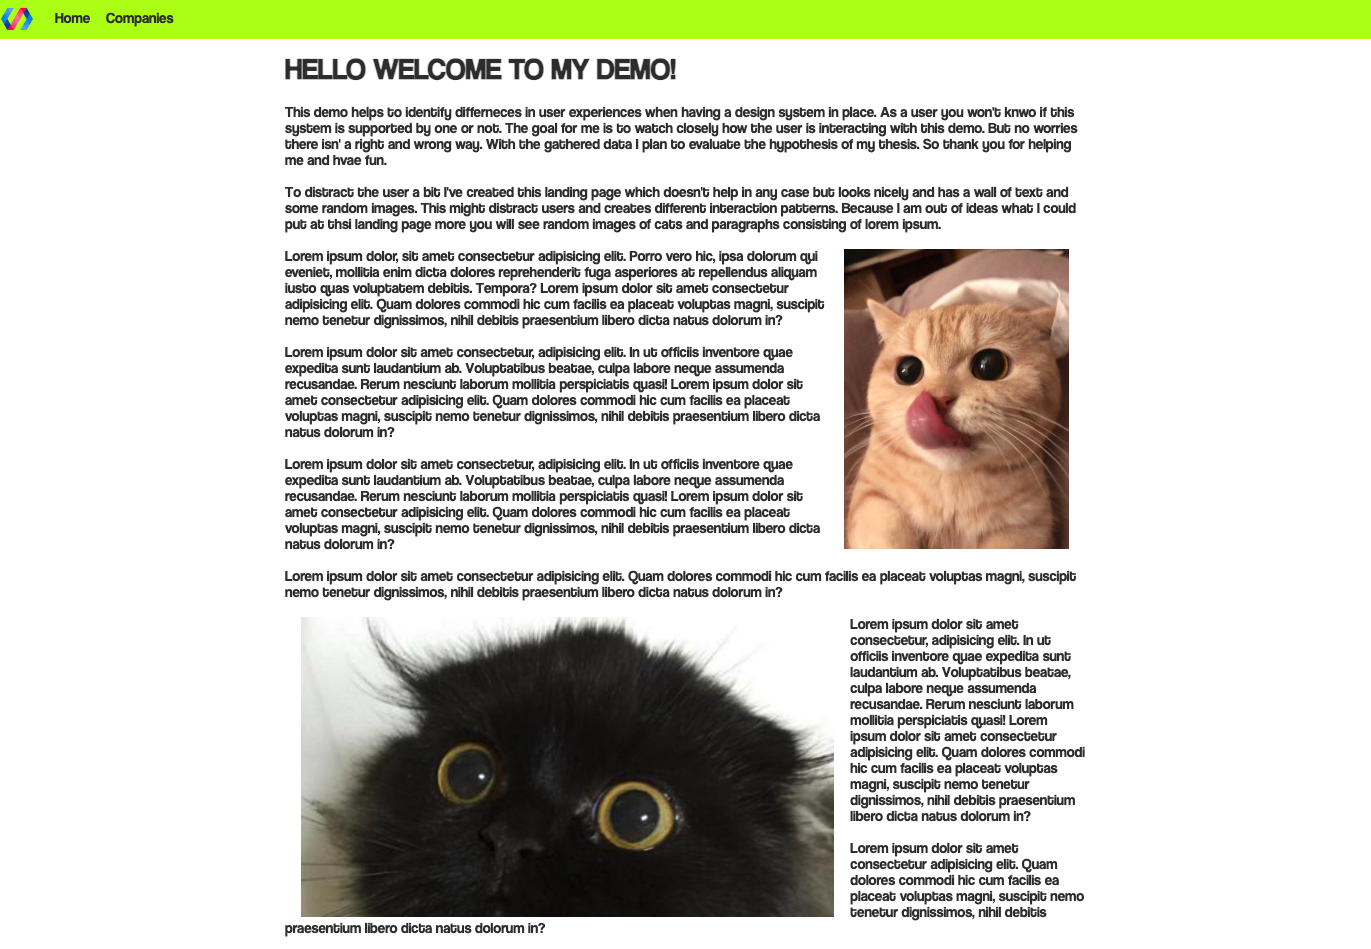
\includegraphics[width=\linewidth, draft=false]{images/demo_view_landing_page.png}}
    \caption{Landing page of test applications}
    \label{landing_page}
\end{figure}
The first view (Figure \ref{landing_page}) is the landing page when the user starts the test run. Here the user will find a navigation bar, which is also included in the other two views, to navigate through the application. The main goal of this view is to distract the user. Long paragraphs with sample texts and cat photos should draw the user's attention. After all, the user is supposed to navigate to the second view, the data table, via the upper navigation bar. When the user clicks on "Companies", a redirection to the second view is triggered. \\
\newpage
In the second view (Figure \ref{data_table}), the user sees a data table with entries from various companies. Besides the company name, the user finds the current status of the company and a description in the table. However, the description is also a Lorem ipsum without any relevance. Finally, the user finds a button labeled "Add +" at the top right of the data table. This button leads him to the third view.  \\

\begin{figure}[htbp]
    \centerline{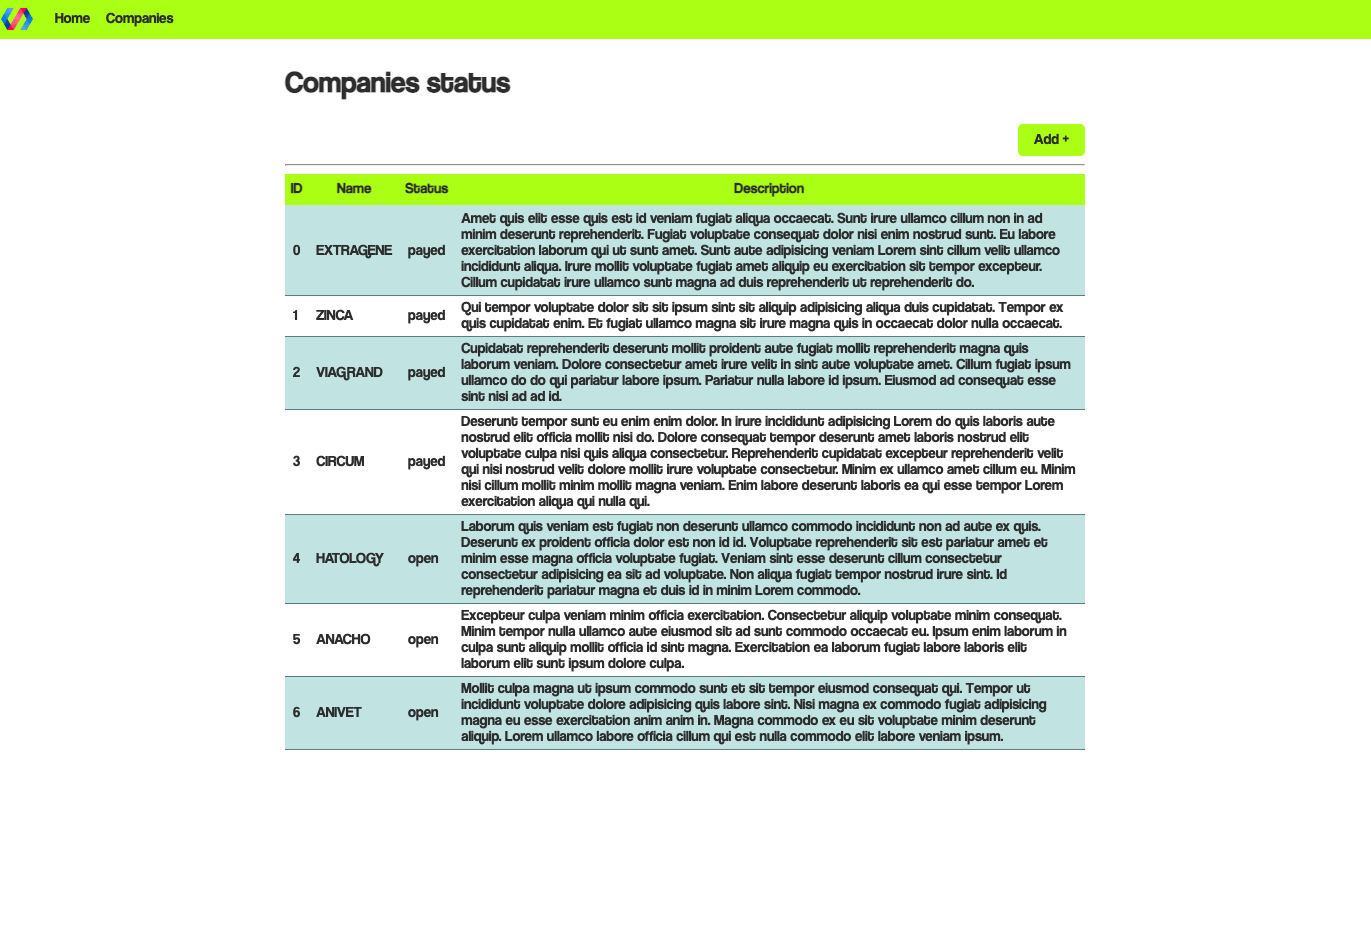
\includegraphics[width=\linewidth, draft=false]{images/demo_view_data_table.png}}
    \caption{Data table page of test applications}
    \label{data_table}
    \end{figure}
The last view (Figure \ref{adding_form}) of the sample applications shows a form for adding new data to the table. The form has three inputs for each value corresponding to the table from the second view. All inputs are simple text inputs with no restriction or validation of the inputs. In a real scenario, there would be validation, but due to the limited time frame of this elaboration, it omits this feature. At the bottom of the form, the user sees a button to save the form. This button is disabled until all input fields are filled have a value. 
\begin{figure}[htbp]
    \centerline{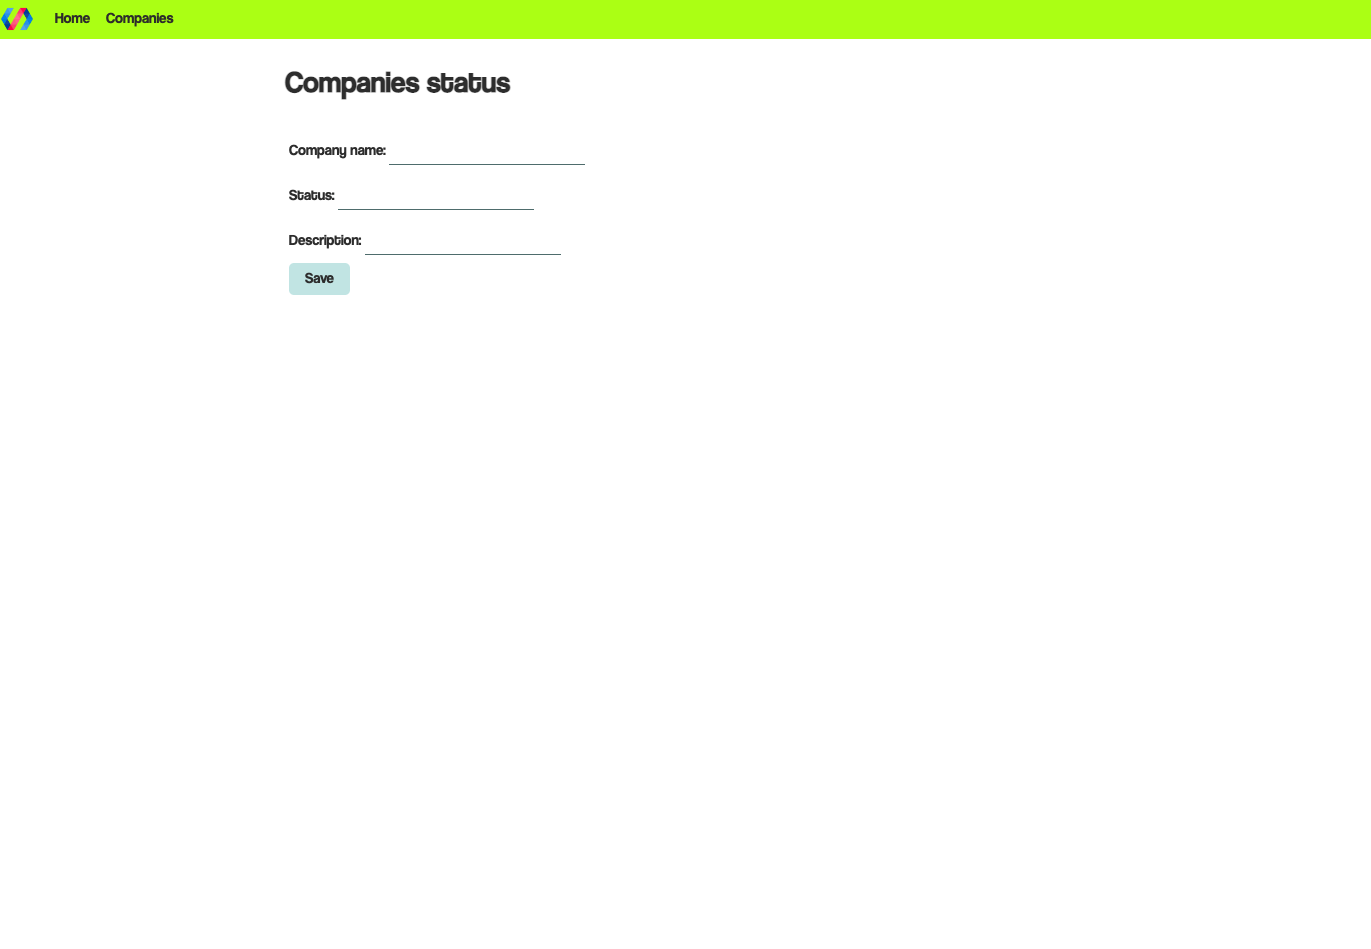
\includegraphics[width=\linewidth, draft=false]{images/demo_view_form.png}}
    \caption{Data adding view of test applications}
    \label{adding_form}
    \end{figure}
\\
Both applications have not only the same views but also the same technology stack. They use Svelte, a library for building web applications with a small package size. According to the starter guide, we use Rollup as a bundling and compilation tool. So both applications do not differ in terms of technology and build steps. \cite{svelte_svelte_nodate} \\
The only difference between the two systems is the implementation details. The following chapters will explain each application's structure and how views are created with and without \ac{SDS}.
\subsubsection{Application using \ac{SDS}}
The first step summarizes how to use the \acl{SDS}. Next, the application must import the code that adds the components from the design system. In this case, the system contains the bundle described in \ref{SDS_build_and_integration}.
The  \texttt{main.ts} file imports the bundle files. Finally, the rollup configuration defines the  \texttt{main.ts} files as an entry files. \\
\lstinputlisting[linerange={1-9},firstnumber=1,caption={Bootstrapping of Svelte application with \ac{SDS}},label=BootstrappingAppSDS]{../Code/sds-demo-app/src/main.ts}
As seen in Listing \ref{BootstrappingAppSDS}, the bootstrapping of the Svelte application is performed here by creating the Svelte App component and appending it to the body. Also, in lines 2 and 3, the SDS bundle Javascript and \ac{CSS} are imported. The import adds the design system components and their styles to the application. Now it is possible to use all the web components within the application via the \ac{HTML} tags defined by \ac{SDS}. \\

After successfully bootstrapping the application, the next step is to look at the Svelte components and how they build the given views. Since the \texttt{App.svelte} component only bootstraps the application and initializes the router, the component does not need further investigation. Therefore, according to the routing details, the next component to be loaded is \texttt{Main.svelte}. \\
The Main component is responsible for displaying the navigation bar, which is visible at the top of each displayed view. In addition, it contains a content placeholder where other components are displayed.  The component's code shows the usage of web components from the  \ac{SDS}. Lines 7-11 in Listing \ref{MainSvelteSDS} use the navigation bar (\texttt{<saas-navbar>}) and the corresponding navigation bar items (\texttt{<saas-navbar-item>}).
\lstinputlisting[linerange={1-14},firstnumber=1,caption={Main.svelte with \ac{SDS}},label=MainSvelteSDS]{../Code/sds-demo-app/src/components/Main.svelte}
The component takes advantage of the functionality of slots by inserting elements into the navbar component. The web component takes care of the corresponding display at the top. The Navbar elements inside ensure that the declared navigation links show up with the correct styles defined by the design system. A special feature in line 8, Listing \ref{MainSvelteSDS} is the \texttt{<img>} element. This \ac{HTML} element is responsible for displaying the logo in the upper left corner. The element has a special property called "slot". Its value is "logo". The web component of the navigation bar recognizes this slot definition and inserts the image with the common styles in the navigation bar. \\
Below the code for the navigation bar, lines 12-14, Listing \ref{MainSvelteSDS}, contain the code for displaying the application's content. In addition to the navigation bar web component, the design system also provides the content component. It uses the same logic as the navigation bar by providing a placeholder for elements within that component and applying styles to the content contained within the web component. Adjustable by design token within the SDS. The \texttt{<Router>} tag within the content is an imported Svelte component that handles the display of the content according to the visited route. \\
For example, one route that is the start of the test is the landing page.The Svelte component \texttt{Home.svelte} represents this page. This component consists only of a few paragraphs and images to distract the user. Therefore, it is not necessary to go into details here. The final result of the view is visible in Figure \ref{landing_page}.\\
An essential component in this comparison is \texttt{Data.svelte}. As the name suggests, this component manages the view of the data table shown in Figure \ref{data_table}. In addition, however, the component's code manages the view of the data table and the view of the data entry form shown in Figure \ref{adding_form}. \\
\lstinputlisting[linerange={84-90},firstnumber=84,caption={Data.svelte with \ac{SDS} table implementation},label=DataSvelteSDSTable]{../Code/sds-demo-app/src/components/Data.svelte}
SDS provides a web component for data tables, visible in in line 89 in Listing \ref{DataSvelteSDSTable}. In order to display the data in the table, two properties are mandatory. 
First, as the name implies, the header property manages the \texttt{header} displayed in the table.  The \texttt{hedaer} object defines a mapping of keys of the table data to the string values that show up as table headers. \texttt{myArray} is the data object handed into the data property of the table web component. Accordingly, the second property is the data input for the table. The data structure of the array should match the data keys defined in the header object so that the data objects within the array match the table headers. \\
Figure \ref{data_table} shows a button at the top of the table. The code snippet also adds the button. Lines 85-87 show the code for the added button. As with the table component, the design system provides a button component thatSection \ref{sds_button} introduced. The \texttt{on:click} property is an indicator of an event listener in Svelte. In this case, a click listener. The event property connects to the \texttt{addEntry} function within the \texttt{Data.svelte} component. This function toggles the boolean variable \texttt{isAddEntry} to \texttt{true}. When the variable changes, the if statement on line 84 is \texttt{false} and activates the else block at line 90. \\

As described in the flow above, the else-block consists of elements to create the view of Figure \ref{adding_form}, the form view. The code snippet looks like this:
\lstinputlisting[linerange={90-100},firstnumber=90,caption={Data.svelte with \ac{SDS} form implementation},label=DemoSvelteSDSForm]{../Code/sds-demo-app/src/components/Data.svelte}
The standard form element between lines 91 and 99 contains the form inputs and a "Save" button. Like the table and the buttons, the form input fields are web components of the design system. The inputs have custom properties for setting the label and its ID to ensure appropriate accessibility. A unique feature of this web component is the custom event for a value change. For example, in line 92, Listing \ref{DemoSvelteSDSForm}, the input receives an event object through this value event and deconstructs the event object to access its details. These details include the changed value of the input field. The newly created data object assigns this value to itself. \\
After all input fields have set a value in the new data object, the "Save" button changes its property \texttt{disbaled} to \texttt{false} and allows click events.Finally, the freshly created object is attached to the data table array with a final click on the button and appears at the bottom. This walkthrough shows all the possibilities of the first test system, and the next section explains the other variant without using the \ac{SDS}. 

\subsubsection{Application not using \ac{SDS}}
One of the main goals is to have a similar application with the same capabilities but not use the design system. So it is necessary to recreate the application from the previous section without using its components. \\
This application uses the same technical stack as the first demo system to avoid significant technical differences between both systems. The bootstrapping of the application looks the same. Listing \ref{MainSvelteSDS} shows it but without the import of SDS code and styles. The application runs and uses Svelte components to create the views described above. \\

As before, a detailed look at the App.svelte is unnecessaryas it is only where the \ac{SPA} initializes the routing. So instead, the first code is in the \texttt{Main.svelte} component to see how this type of application constructs the navigation bar and router content. 
\lstinputlisting[linerange={1-17},firstnumber=1,caption={Main.svelte without \ac{SDS}},label=MainSvelteNormal]{../Code/normal-demo-app/src/components/Main.svelte}
Besides using fewer lines of code compared to Listing \ref{MainSvelteSDS}, the main difference is that no custom web components build the navigation bar or its elements. Here, web standards help by using the correct \ac{HTML} tags to describe specific areas of the application. \\
For example, the navigation bar uses the \texttt{<nav>} tag in lines 6-12 to enclose an unsorted list that tells the browser that this is a navigation area for the application. The same construct of an \ac{HTML} tree was used in the \ac{SDS} demo but hidden behind web components, so the developer does not have to think about it when implementing a navigation bar. \\
The same concept is visible below the navigation bar code in lines 13-17, Listing \ref{MainSvelteNormal}. Here the main content is encapsulated by a \texttt{<main>}, which is also an indicator for the browser. \\
Nevertheless, the part that is not visible in Listing \ref{MainSvelteNormal} and gives the \ac{HTML} element this good look is the styling. Since the \ac{SDS} components are built based on best practices from across the field, no one has to develop a new styling concept and fix style glitches that may occur during development. 
\lstinputlisting[linerange={18-48},firstnumber=18,caption={Main.svelte styles without \ac{SDS}},label=MainSvelteNormalStyles]{../Code/normal-demo-app/src/components/Main.svelte}
As seen in Listing \ref{MainSvelteNormalStyles}, many styles have fixed values for style rules. As in line 23, it is possible to define design tokens in an application and use them in place of the fixed values. However, this usage does not guarantee that the application uses them every time. In an existing design system, components ensure the usage of the defined design tokens. \\
Nevertheless, it is not just consistency that is important. It is also the time required to rewrite those lines of code repeatedly for each new application. Ultimately, this code snippet produces the same view of Figure \ref{landing_page} as in the other demo, but it takes a lot more thinking to get to this result.  \\

The demo project without using the SDS also creates the second view shown in Figure 8, the data table. The project contains a svelte component named \texttt{Data.svelte}, as in the previous section. As in the other application, Data.svelte consists of two views simultaneously. \\
The responsible code snippet looks like this:
\lstinputlisting[linerange={86-92},firstnumber=86,caption={Data.svelte without \ac{SDS} table implementation},label=DataSvelteNormalTable]{../Code/normal-demo-app/src/components/Data.svelte}
At first glance, the component code looks similar to that in Listing \ref{DataSvelteSDSTable}. However, the names of the \texttt{<SvelteTable>} table component and the \texttt{<SvelteButton>} button component hint at of how the application constructs these components. Both Svelte components replicate the logic familiar from the Web components presented earlier. \\
One might ask why it is necessary to build web components when it is possible to build them this way and ensure no style inconsistencies. The answer is that this works for an application with this specific technology stack to reuse these Svelte components. If one is okay with using a limited technology stack to ensure the use of a specific component library, then that is fine. However, the reality is that there are many different frameworks, each with a specific component implementation.\\
In this case, the application builds each component and uses it here, as shown in lines 88 and 91 in Listing \ref{DataSvelteNormalTable}. \\
For example, \texttt{<SvelteButton>} represents the button in the upper right and receives an event to switch to the third view, the form view.Because it is a standalone component, the buttons' styles are not in the \texttt{Data.svelte} component's code but in the button's code. In addition, as explained with the navigation bar, the button styles are defined as fixed values, not as design tokens that a design system would provide. These fixed values cause difficulties when changing the appearance of multiple components with a single value change. \\
The same rules apply to the table component just presented. Therefore, both properties are responsible for ending up in the table in Figure \ref{data_table} as the render result. This explanation sets up the second view and a click on the button reveals the third view (Figure \ref{adding_form}). \\

As the last detail, it is time to look at the code that creates the form for entering a new data object into the table. These elements are visible if the if-statement from line 86, Listing \ref{DataSvelteNormalTable}, results in a \texttt{false} statement, ergo, \texttt{isAddEntry} is \texttt{true}. The result is the block of code that displays the input fields in the browser:
\lstinputlisting[linerange={92-99},firstnumber=92,caption={Data.svelte without \ac{SDS} form implementation},label=DataSvelteNormalForm]{../Code/normal-demo-app/src/components/Data.svelte}
A new svelte component can be seen in lines 94-96, Listing \ref{DataSvelteNormalForm}. As the name \texttt{<SvaleteInput>} indicates, this component is a text input field for the form. However, in addition to the familiar property of indicating an input by specifying a string value, there is a particular Svelte property. The keyword \texttt{bind} indicates a two-way data binding in Svelte. A two-way data binding means the assigned value is available in the component. Therefore, if this variable changes its value within the component, it also reflects the changes outside of it. \\  
Recalling the code snippet from the web component implementation (Listing \ref{DemoSvelteSDSForm})to compare both versions shows it is impossible to \texttt{bind} a value and the event output of a custom web component. In this case, it was necessary to listen to the event manually to get the details. So maybe it is worth avoiding using web components in frameworks because of the lack of such features. \\
With the addition of the button component in line 97, Listing \ref{DataSvelteNormalForm}, the implementation of the form to submit new data to the data field is complete. As with the web component implementation, the button has a \texttt{disabled} property that blocks click events when set to true. Validating the form's input values will either disable the button or not. \\


This last functionality concludes the details of the implementation of the demo systems used to test the SDS. The next step is to examine the test case to test the design system. 
% View 3 
\subsection{Test case}\label{text_case}
A test case helps determine whether a design system created for a common purpose helps users work better with an application. In this elaboration, one test case is performed with two test applications to get better test results. One with \ac{SDS} implemented and one without \ac{SDS}.  \\
Since both systems are visually identical, it is impossible to test them with the same person. The tester would already know how to operate and navigate through the test system by the second run. Therefore, it is necessary to perform a reasonable number of test runs on both systems with approximately the same type of person. By person type in this elaboration is meant what a person does in his daily job, e.g., accountant.  \\
The test provides two results for this elaboration. First is the observation of the test execution for each person. The purpose of this observation is to see how the subject responds to the navigation structure of the web page. How the subject navigates to the next page? Which controls do the users use, whether mouse, keyboard, or other unique controls? Testing is done in person to capture emotions and reactions to the content's appearance and disappearance. At the end of a test run, the subject is asked for additional feedback on the application just tested. With this subjective input, it is possible to assess whether the use of \ac{SDS} affects anything. \\
In addition, the test uses time measurement points in each application. These points provide objective feedback about the time spent on particular views or actions.Furthermore, the applications locate the measurement points in the same place, so comparing both types is possible. In this way, it is feasible to obtain unbiased data for evaluation. \\
In preparation for the test runs, the two applications with and without implementation of the design system are globally available as static web pages. The test person opens one of the two applications and finds a description of the test procedure. The description informs the user that the following application might implement a design system. After the brief introduction, the first view explains the three test steps to the user:

\begin{enumerate}
    \item Navigate to the data table containing the records of different companies.
    \item Find the action to create a new data record.
    \item Fill out the form and submit a new entry.
\end{enumerate}

Since users are not given any instructions on navigating to the data table or with what details to fill in the new record, users are free to explore the demo application. The test steps are intentionally vague to allow users to develop their patterns in their interaction.  \\
After reading all the instructions, the applications will ask the users to start the test by clicking the "Start" button below. This interaction will trigger the first measurement point, which is the start of the demo. \\
The interaction also takes the users to the landing page shown in Figure \ref{landing_page}. On this page, users need to figure out how to navigate to the companies' data table. By scanning the view, they should figure out how to use the navigation bar at the top to navigate to the Companies page. When the user clicks on the navigation bar, they will navigate to the data table view and the second measurement point will be triggered. Again, the memory stores the measured time needed. \\
In the second view (Figure \ref{data_table}), the user sees the data table containing the entries. To add a new entry to the data table, the user must click on the "Add +" button in the upper right corner of this view. With pressing the button, the view changes to the third view (Figure \ref{adding_form}). As with the last view change, the user triggers a new measurement point, and the time data stores it in the memory.  \\ 
In the last view, the user fills in the given form and clicks on "Save" to store the data in the table. The action again triggers and saves a measurement point for the test. When saving the new data unit in the table, the user is navigated back to the table and automatically downloads a JSON file containing all the measurement points described. This JSON file is then sent to the author of this elaboration to collect the measurement of each participant. \\

By collecting all the measurement data and observing the user behavior during the interaction, this test case provides much data for evaluation. These final words conclude this chapter and lead to the next chapter, presenting the test results and their evaluation. 
% \subsection{Execution}